\documentclass[tikz,border=6pt]{standalone}
\usepackage{amsmath,amssymb}
\usepackage{xcolor}
\definecolor{accent}{HTML}{A13D2C}
\definecolor{accent2}{HTML}{2B5F6B}
\definecolor{muted}{HTML}{5A564F}
\definecolor{panel}{HTML}{F8F6F0}
\definecolor{linecol}{HTML}{D8D2C4}
\definecolor{astroblue}{HTML}{1B4F72}
\definecolor{sunyellow}{HTML}{E8A33D}
\definecolor{colthree}{RGB}{60,140,80}
\definecolor{dust}{HTML}{8C6D4F}
\usetikzlibrary{calc,arrows.meta}
\usepackage[T1]{fontenc}\usepackage{newpxtext,newpxmath}  % same fonts as the notes
\begin{document}
% Schematic cross-section of an active nucleus (not to scale): black hole, accretion disk,
% broad-line clouds, dusty torus, narrow-line clouds, two jets, and three sight lines.
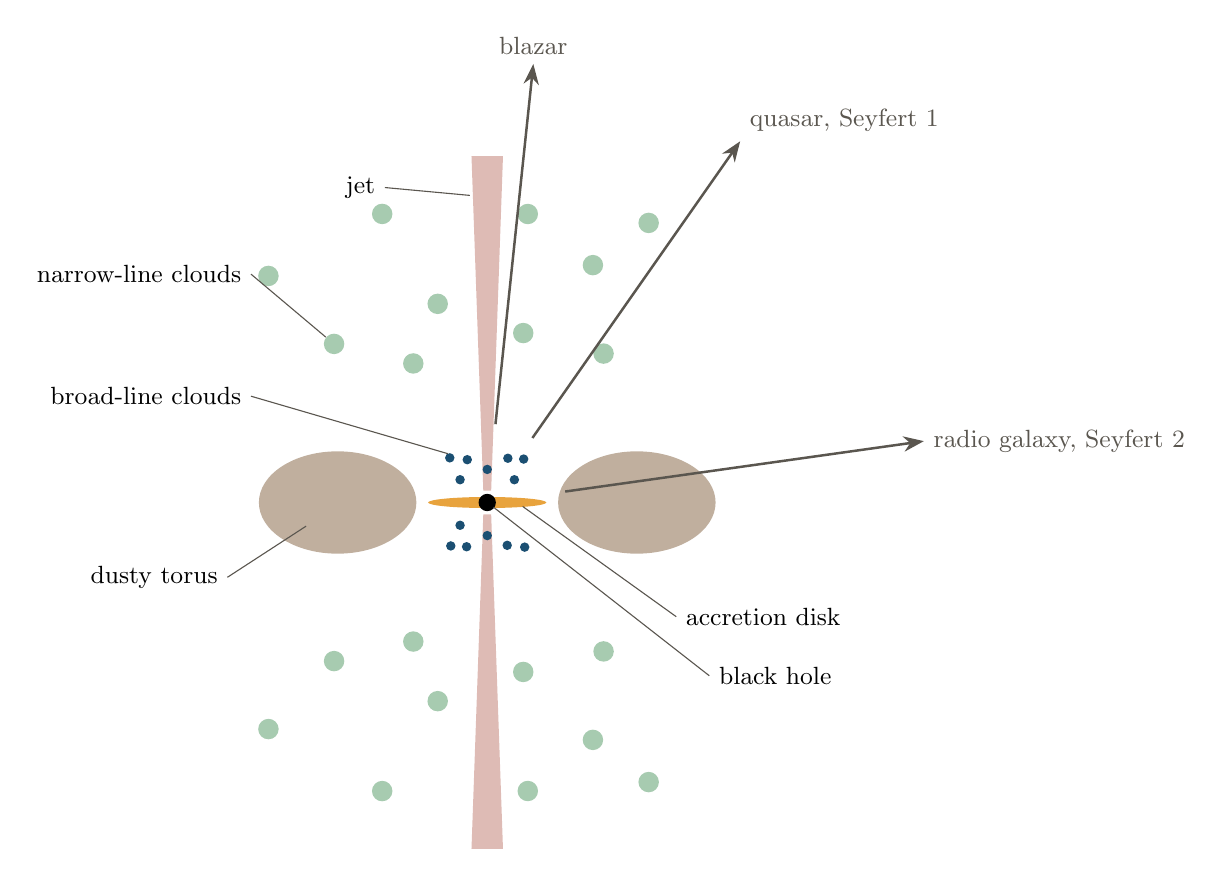
\begin{tikzpicture}[x=1cm,y=1cm, >={Stealth[length=2.6mm]}, font=\small]
  % jets
  \fill[accent!35] (-0.05,0.15) -- (-0.2,4.4) -- (0.2,4.4) -- (0.05,0.15) -- cycle;
  \fill[accent!35] (-0.05,-0.15) -- (-0.2,-4.4) -- (0.2,-4.4) -- (0.05,-0.15) -- cycle;
  % narrow-line clouds, in two cones about the axis
  \foreach \ang/\rad in {-38/2.4, -24/3.3, -12/2.2, -30/4.1, -8/3.7, 14/2.6, 20/3.9, 44/2.8, 44/4.0, 28/2.0}{
    \fill[colthree!45] ($(0,0)+(90+\ang:\rad)$) circle (0.13);
    \fill[colthree!45] ($(0,0)+(-90-\ang:\rad)$) circle (0.13);
  }
  % dusty torus, cut through
  \fill[dust!55] (-1.9,0) ellipse (1.0 and 0.65);
  \fill[dust!55] (1.9,0) ellipse (1.0 and 0.65);
  % broad-line clouds, close to the hole
  \foreach \ang/\rad in {-50/0.45, -25/0.62, 0/0.42, 25/0.6, 50/0.45, -40/0.72, 40/0.74}{
    \fill[astroblue] ($(0,0)+(90+\ang:\rad)$) circle (0.06);
  }
  \foreach \ang/\rad in {-50/0.45, -25/0.62, 0/0.42, 25/0.6, -40/0.72, 40/0.74}{
    \fill[astroblue] ($(0,0)+(-90+\ang:\rad)$) circle (0.06);
  }
  % accretion disk and hole
  \fill[sunyellow] (0,0) ellipse (0.75 and 0.07);
  \fill[black] (0,0) circle (0.11);
  % sight lines, light travelling from the nucleus to three observers
  \foreach \ang/\lab in {6/{blazar}, 35/{quasar, Seyfert 1}, 82/{radio galaxy, Seyfert 2}}{
    \draw[->, muted, line width=0.9pt] ($(0,0)+(90-\ang:1.0)$) -- ($(0,0)+(90-\ang:5.6)$);
  }
  \node[anchor=south, muted] at ($(0,0)+(84:5.6)$) {blazar};
  \node[anchor=south west, muted] at ($(0,0)+(55:5.6)$) {quasar, Seyfert 1};
  \node[anchor=west, muted] at ($(0,0)+(8:5.6)$) {radio galaxy, Seyfert 2};
  % labels of the parts, with leader lines
  \draw[muted, thin] (-1.3,4.0) -- (-0.22,3.9);
  \node[anchor=east] at (-1.3,4.0) {jet};
  \draw[muted, thin] (-3.0,2.9) -- (-2.05,2.1);
  \node[anchor=east] at (-3.0,2.9) {narrow-line clouds};
  \draw[muted, thin] (-3.0,1.35) -- (-0.5,0.62);
  \node[anchor=east] at (-3.0,1.35) {broad-line clouds};
  \draw[muted, thin] (-3.3,-0.95) -- (-2.3,-0.3);
  \node[anchor=east] at (-3.3,-0.95) {dusty torus};
  \draw[muted, thin] (2.4,-1.45) -- (0.45,-0.05);
  \node[anchor=west] at (2.4,-1.45) {accretion disk};
  \draw[muted, thin] (2.82,-2.2) -- (0.08,-0.06);
  \node[anchor=west] at (2.82,-2.2) {black hole};
\end{tikzpicture}
\end{document}
